
\documentclass[a4paper]{article}
\setlength{\oddsidemargin}{0 in}
\setlength{\evensidemargin}{0 in}
\setlength{\topmargin}{0 in}
\setlength{\textwidth}{6.5 in}
\setlength{\textheight}{8.5 in}
\setlength{\headsep}{0 in}
\setlength{\parindent}{0 in}
\setlength{\parskip}{0.1 in}

%
% ADD PACKAGES here:
%

\usepackage{amsmath,amsfonts,graphicx,amssymb,ulsy} 

%\usepackage[backend=bibtex]{biblatex}

\usepackage{tikz}   %these go together to make frameworks
\usetikzlibrary{arrows,shapes} 
\usetikzlibrary{matrix} 
\usepackage{verbatim}   

\usepackage{algorithm} %pseudo code needs these
\usepackage[noend]{algpseudocode}
\usepackage{setspace}
\let\Algorithm\algorithm
\renewcommand\algorithm[1][]{\Algorithm[#1]\setstretch{1.4}}


\usepackage{hyperref}

\usepackage{float}

% The following commands set up the lecnum (lecture number)
% counter and make various numbering schemes work relative
% to the lecture number.
%
%\newcounter{lecnum}
%\renewcommand{\thepage}{\thelecnum-\arabic{page}}
%\renewcommand{\thesection}{\thelecnum.\arabic{section}}
%\renewcommand{\theequation}{\thelecnum.\arabic{equation}}
%\renewcommand{\thefigure}{\thelecnum.\arabic{figure}}
%\renewcommand{\thetable}{\thelecnum.\arabic{table}}

%
% The following macro is used to generate the header.
%
\newcommand{\lecture}[4]{
   \pagestyle{myheadings}
   \thispagestyle{plain}
   \newpage
   %\setcounter{lecnum}{#1}
   \setcounter{page}{1}
   \noindent
   \begin{center}
   \framebox{
      \vbox{\vspace{2mm}
 %   \hbox to 6.28in { {\bf Graph Theory
%		\hfill Combinatorics} }
       \vspace{2mm}
       \hbox to 6.28in { {\Large \hfill Gatekeeping in Campaign Contribution Networks \hfill} }
       \vspace{2mm}
       \hbox to 6.28in { {\it June 2016  \hfill James David Moffet III and Lihan Yao} }
      \vspace{2mm}}
   }
   \end{center}
}
%
% Convention for citations is authors' initials followed by the year.
% For example, to cite a paper by Leighton and Maggs you would type
% \cite{LM89}, and to cite a paper by Strassen you would type \cite{S69}.
% (To avoid bibliography problems, for now we redefine the \cite command.)
% Also commands that create a suitable format for the reference list.
\renewcommand{\cite}[1]{[#1]}
\def\beginrefs{\begin{list}%
        {[\arabic{equation}]}{\usecounter{equation}
         \setlength{\leftmargin}{0.5truecm}\setlength{\labelsep}{0.4truecm}%
         \setlength{\labelwidth}{1.6truecm}}}
\def\endrefs{\end{list}}
\def\bibentry#1{\item[\hbox{[#1]}]}

%Use this command for a figure; it puts a figure in wherever you want it.
%usage: \fig{NUMBER}{SPACE-IN-INCHES}{CAPTION}
%\newcommand{\fig}[3]{
%			\vspace{#2}
%			\begin{center}
%			Figure \thelecnum.#1:~#3
%			\end{center}
%	}
% Use these for theorems, lemmas, proofs, etc.
\newtheorem{theorem}{Theorem} %[lecnum]
\newtheorem{lemma}[theorem]{Lemma}
\newtheorem{proposition}[theorem]{Proposition}
\newtheorem{claim}[theorem]{Claim}
\newtheorem{corollary}[theorem]{Corollary}
\newtheorem{definition}[theorem]{Definition}
\newtheorem{exercise}[theorem]{Exercise}
\newtheorem{observation}[theorem]{Observation}
\newenvironment{proof}{{\bf Proof:}}{\hfill\rule{2mm}{2mm}}

%\newenvironment{solution}{ Solution: }{\hfill\rule{2mm}{2mm}}

% **** IF YOU WANT TO DEFINE ADDITIONAL MACROS FOR YOURSELF, PUT THEM HERE:

\newcommand\E{\mathbb{E}}
\newcommand{\Var}{\mathrm{Var}}





\begin{document}
%FILL IN THE RIGHT INFO.
%\lecture{**LECTURE-NUMBER**}{**DATE**}{**LECTURER**}{**SCRIBE**}
\lecture{1}{August 24}{Aarti Singh}{scribe-name}

%\section*{Gatekeeping in Campaign Contribution Networks}

During this year's, for lack of a better word, unique cycle of US presidential campaigns, we have a ballot of extremely diverse candidates, whose campaign funding strategies are even more diverse than the candidates themselves. We hope that all of the spectacle can be put to some use as a frame for investigating the influence of individuals in campaign contribution networks, specifically the exercise of veto power over campaign viability, or what we term "gatekeeping" behavior. 

Our research topic originated from a self-evident observation: a ballot of candidates chosen by a small percentage of voters is less democratic than a ballot of candidates chosen by a large percentage of voters. Following from this observation, we decided to investigate contribution networks as a determining factor in the selection of viable candidates in US-style elections.

How do we identify the gatekeepers of campaign viability, and what properties do they have? As a computational problem, we define a set of gatekeepers as the minimal number of nodes whose removal from the network produces components which no longer contain enough resources to surpass some threshold of viability. We hypothesized, and can now observe, that both high "contribution" value (vertex weight) and crucial topological position determine the gatekeeper nodes' collective ability to destroy the viability of every "campaign" (subgraph) in the network. 

We hope to develop a computationally-efficient way to describe gatekeeping behavior in real world networks. We believe that modeling this phenomenon may yield insights for domains in which a critical mass of resources is required to change a given state. 

\section*{Zachary's Karate Club Example}

In our preliminary investigation, we observe relationships between three parameters and the relative size/composition of the gatekeeper set: distribution of resources \ref{di} (as vertex weights), threshold of viability \ref{th} (as sum of weights in a component) and network density \ref{de}. We can computationally discover gatekeeper sets and have done so for a series of graphs with a variety of values for these parameters. 

The main takeaway is that distribution swamps all other parameters in terms of influencing GP set size. However, benefits of mitigating wealth inequality begins to diminish well before the distribution resembles egalitarian society. The difference between our medium and flat distributions is almost negligible when compared to the punishing version. For reference, the distribution curve for a punishing can be best fit by $y=x^300$ and medium nearly being $y=x^70$. The medium distribution still depicts a harsh distribution of wealth even though the marginal return on decreasing inequality is basically gone. From the authors' experiences working with electoral campaigns, a best fit of $x^300$ is our estimate for the actual distribution.

Higher threshold, unequal distribution and decreasing density implies a more autocratic gatekeeping behavior, quantitatively we mean that smaller GP set size are exhibited.

This observation holds regardless of how the other parameters are manipulated. 

\begin{figure}[ht!]
\centering
\includegraphics[width=250mm, height = 100mm,angle = 90]{Density.jpg}
\caption{Varying Edge Density \label{de}}
\end{figure}

\begin{figure}[]
\centering
\includegraphics[width=250mm, height = 100mm, angle  = 90]{Threshold.jpg}
\caption{Varying Threshold \label{th}}
\end{figure}

\begin{figure}[]
\centering
\includegraphics[width=250mm, height = 100mm,angle = 90]{Distribution.jpg}
\caption{Varying Distribution \label{di}}
\end{figure}

\section*{Computing Gatekeepers}

As a computational problem, let $G = (V,E)$ be a simple, vertex weighted graph. Call the weight function $w: V \rightarrow \mathbb{R}$. Lastly, attribute to $G$ some $t \in \mathbb{Z}$ called the threshold.  

\begin{definition}
If for some $X \subseteq V$ we have that $G[X]$ is connected and \[\sum_{v\in X}w(v) \geq t\] then $X$ is a {\bf viable set}.
\end{definition}

\begin{definition}
If after removing $K \subseteq V$ from $G$, $G[V-K]$ contains no viable sets, and $K$ is size minimal with respect to this property, we call $K$ a {\bf gatekeeper set}
\end{definition}

The union of gatekeeper sets are called gatekeepers. Below are two techniques for the computation of such GP sets, one by sophisticated sorting of vertex combinations of certain size, and another by measure and conquer, where we explore the tree of possible cut unions and stop whenever a terminal condition, called filters, are met.  

\begin{algorithm}
\caption{Brute Force}\label{euclid}
\begin{algorithmic}
\Function{CompScore}{graph}
\For{{$x \in V$}}
\State {$E_c$ $\gets$ compute and normalize eigenvector centrality}
\State {$w_n$ $\gets$ normalize vertex weight}
\State {composite score of x, $C_s$ $\gets$ $E_c + w_n$}
\EndFor
\EndFunction

\Function{GetGPSet}{graph, threshold}

\For{$i \leq |V| $}
\State Arrange vertices of $V$ according to $C_s$ 
	\State Create generator $g_i$ which yields all ($|V|$ choose $i$ vertex combinations) according to arrangement
	\State Counter $\gets$ 0 
	\State Terminal-Value $\gets {\binom{|V|}{i}} 0.1$
	\State $C_i$ $\gets g_i$
	\If{$G[V-C_i]$ has no viable components}
	\State record $C_i$ in array
	\State terminate after computing this $i$ value
	\EndIf
	\If {Counter = Terminal-Value}
	\State break
	\EndIf
	
\EndFor
\Return GP sets

\EndFunction
\end{algorithmic}
\end{algorithm}

\begin{algorithm}
\caption{Measure and Conquer}\label{euclid}
\begin{algorithmic}
\Function{DEL-TIL-UNVI}{graph, threshold}

\State $D = \{\}$ \Comment{Stores vertices to be deleted}  
      \While{$\sum_{v\in G}w(v) \geq  $ threshold} %\Comment{We have the answer if r is 0}
      	\State $D$ $\gets$ highest weight vertex
        \State Delete highest weight vertex 
      \EndWhile\label{euclidendwhile}
\Return $D$ 
%
%\While{$\sum_{v\in G} \geq  $ threshold}
%\State Delete highest value vertex  
%\Endwhile 
\EndFunction

\Function{GEN-CUT}{graph, size}
\State {\bf yield } cut union of graph whose cardinality is smaller than size
\EndFunction 

\State Component-Hash = \{\}

\Function{FILTER}{graph, threshold}

\If {$\sum_{v\in G}w(v) <  $ threshold}
\State Raise exception 
\EndIf

\State D $\gets$ DEL-TIL-UNVI(graph) \Comment{updated whenever we find a smaller candidate for GP set}

\State Connectivity $\gets$ graph connectivity

\If{Connectivity$ >D$} \Comment{Filter: no cut union smaller than DEL-TIL-UNVI}
	\State Update Component-Hash with $D$
	\State 
	\Return str(*+D)
\EndIf


\Return str(D)



\EndFunction

\State S $\gets$ FILTER(graph, threshold)

\Function{MEA-CON}{graph, threshold}
\If{first digit of FILTER(graph, threshold) is not *}


\For{$C \in$ GEN-CUT(graph, $S-$cardinality of previous cut unions)}
	\State Sum $|C|$ with previous cut unions used to reach this graph component, call it $\Sigma C$
	\State break if $\Sigma C >$ than some $D$ of previous components 
	\State 
	\Comment{We do not consider this $C$ since a smaller GP set would have been possible by taking $D$ some time earlier}
	\State $G_C$ $\gets$ $G[V-C]$
	\For{component of $G_C$}
	\If{component $\in$ Component-Hash}
	\State update Component-Hash
	\State continue
	\EndIf
	
	\State MEA-CON(component) 
	%\State update Component-Hash
	\EndFor
\EndFor

\EndIf

\Function{MAIN}{graph, threshold}

\State MEA-CON(graph, threshold)

\EndFunction



\Return GP-sets

\EndFunction
\end{algorithmic}
\end{algorithm}



\begin{algorithm}
\caption{Percolation}\label{euclid}
\begin{algorithmic}
\For{{$i \in |V|$}}
	
	\Function{GetV}{table}
	%\For{{$x \in V$}}
	%\State {$E_c$ $\gets$ compute and normalize eigenvector centrality}
	%\State {$w_n$ $\gets$ normalize vertex weight}
	%\State {composite score of x, $C_s$ $\gets$ $E_c + w_n$}
	%\EndFor
	\EndFunction
	
	\Function{BuildDigraph}{graph, threshold}
	%
	%\For{$i \leq |V| $}
	%\State Arrange vertices of $V$ according to $C_s$ 
	%	\State Create generator $g_i$ which yields all ($|V|$ choose $i$ vertex combinations) according to arrangement
	%	\State Counter $\gets$ 0 
	%	\State Terminal-Value $\gets {\binom{|V|}{i}} 0.1$
	%	\State $C_i$ $\gets g_i$
	%	\If{$G[V-C_i]$ has no viable components}
	%	\State record $C_i$ in array
	%	\State terminate after computing this $i$ value
	%	\EndIf
	%	\If {Counter = Terminal-Value}
	%	\State break
	%	\EndIf
	%\EndFor
	\Return GP sets
	
	\EndFunction
	
	\Function{FindNbr}{table}
	\EndFunction
	
	\Function{UpdateTable}{table}
		\Function{UpdateV}{}
		\EndFunction
	\EndFunction 
\EndFor 

\end{algorithmic}
\end{algorithm}

\section*{Site Percolation}

A modification of the tree algorithm seen in: {\bf A fast Monte Carlo algorithm for site or bond percolation}. The site percolation algorithm yields a collection of approximate solutions. 

Start with a new directed graph $D_0$ that is initially empty. For a digraph $D_i$ at the $i$th step, vertex random variable $X: V(G)\backslash (V(D_{i-1}) \cup GP) \rightarrow Z^+ $ yields a vertex $v_i$ according to a density value function $f_X$, where $GP$ is the candidate gatekeeper set of this trial (see next section for specifications on $X$ and $f_X$). %define a probability function $p: V(G)\backslash V(D_{i-1}) \cup GP \rightarrow [0,1]$, where $GP$ is the candidate gatekeeper set of this trial. 

%On the $(i+1)$-th step, a vertex $v \in V(G)\backslash V(D_i)$ has probability $p(v)$ of being added to $D_i$ to form $V(D_{i+1})$. 

Upon adding $v_i$, if $N_G(v)\cap V(D_{i-1}) = \emptyset $, that is, the neighbors of $v_i$ in $G$ are not in $D_{i-1}$, add $(v,v)$ to $D_{i}$. Otherwise, $ \forall w \in N_G(v)\cap V(D_{i})$, add $(v,w)$ arcs to $D_{i}$. 

If $v$ sends arcs to one component $C$ in $D_{i}$, there is a unique vertex $r$ in $C$ with a loop. $r$ is retrieved by simply traversing to the root of the directed tree within $C$. $w(r) \leftarrow w(r) + w(v)$ and $w(v) \leftarrow 0$. The node whose weight represent the total value of the component, $r$, is updated after the addition of $v$. A $v$-to-$r$ arc is added to take advantage of "path compression." Path compression makes path traversal faster the next time we have to retrieve the aggregate component value $w(r)$. If $w(r) > T$ in $D_{i+1}$, $v$ is noted as a member of the candidate gatekeeper set $GP$ and $p$ is recalculated for $D_i$. Discard $D_{i+1}$. 

If $v$ has arcs toward multiple components $C_1, C_2, \ldots, C_k$, for the $j$ th component there is an unique vertex $r_j$ with a loop. Pick one such vertex at random, denote it $r^*$. This means in $G$, $v$ is connected to multiple components that will now pool together their values. Add $(v,r^*)$ and move the value within $v$ to $r^*$. Then we amalgamate the numerous component values of $C_1, \ldots C_k$ to designated node $r^*$. First add arcs to $r^*$ from nodes previously representing their own components, i.e. $\{r_1,\ldots,r_k\} - r^*$, then remove all loops in $D_{i+1}$ except $(r^*,r^*)$. 

For the $j$-th component $C_j$, whose value is represented by $w(r_j)$, we have that: $w(r^*) \leftarrow w(r^*)+w(r_j), w(r_j) \leftarrow 0, D_{i+1} - (r_j,r_j), D_{i+1} + (r_j,r^*)$. Likewise, if $w(r^*)>T$ in $D_{i+1}$, $v$ is noted as belonging to $GP$ and $p$ is recalculated for $D_i$. Discard $D_{i+1}$.  

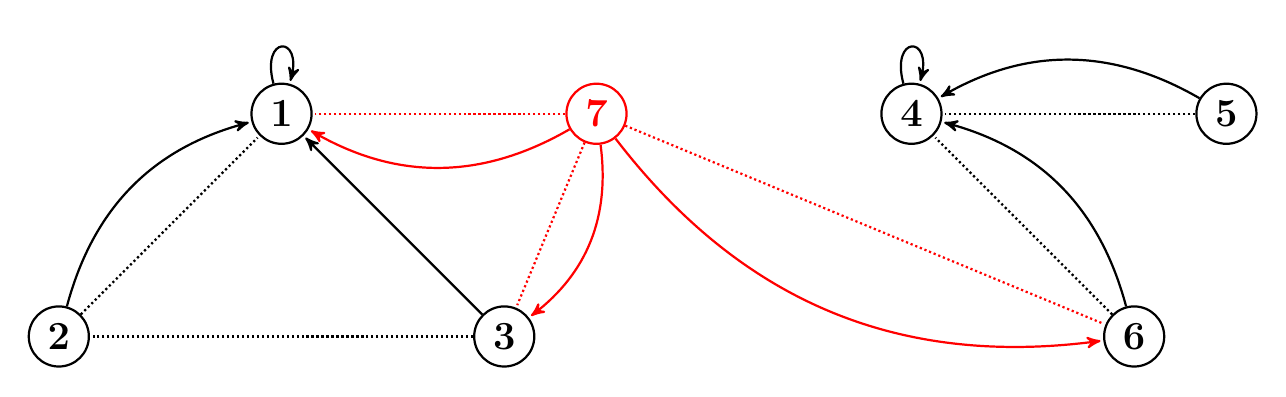
\begin{tikzpicture}[->,>=stealth',shorten >=1pt,auto,node distance=4cm,
                thick,main node/.style={circle,draw,font=\Large\bfseries}]

  \node[main node] (1) {1};
  \node[main node] (2) [below left of=1] {2};
  \node[main node] (3) [below right of=1] {3};

  \node[main node,red] (7) [right of=1] {7};

  \node[main node] (4) [right of=7]{4};
  \node[main node] (5) [right of=4] {5};
  \node[main node] (6) [below right of=4] {6};

  \path
    (1) edge [loop above] node {} (1)
    (2) edge [bend left] node [below]{} (1)
    	edge [densely dotted,-] node[below] {} (1)
    (3) edge node[right] {} (1)
        edge [densely dotted,-] node[below] {} (2)   
        
    (4) edge [loop above] node {} (4)
    (5) edge [bend right]node [left]{} (4)  
    	edge [densely dotted,-] node{}(4)
    (6) edge [densely dotted,-] node [above]{} (4)
    	edge [bend right] node {} (4)    
    
    (7) edge [bend right, red] node [left]{} (6)
    	edge [densely dotted,-,red] node[below] {} (6)
    	edge [densely dotted,-,red] node[below] {} (1)
    (7) edge [bend left, red] node [left]{} (1)
    	edge [bend left, red] node {} (3)
    	edge [densely dotted, -, red] node {}  (3);
    %(1) edge [bend left,red] node {} (4);
    
\end{tikzpicture}


The nodes are labeled according to the order in which they are added. Dashed lines denote edges in original graph $G$. $7$ has connected two components, whose aggregate values are recorded by $w(v_1)$ and $w(v_4)$. In this example,$r^* = v_4$, and $(v_1,v_1)$ will be removed from $D_i$. The value $w(v_1)$, in addition to $w(v_7)$, will be moved to $v_4$. Notice that even though there are only two components, three path traversals must be conducted by $v_7$ in the event that it is connected to three components in $G$. 

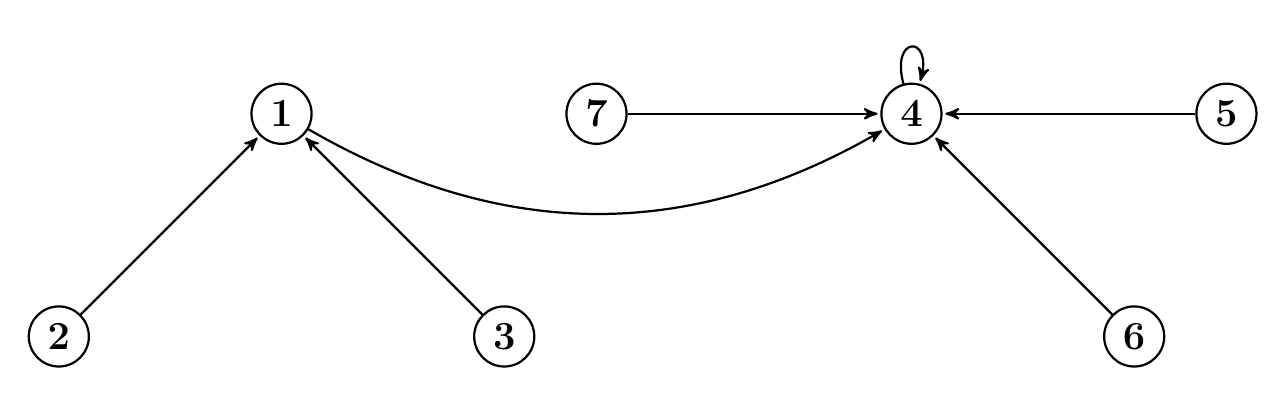
\begin{tikzpicture}[->,>=stealth',shorten >=1pt,auto,node distance=4cm,
                thick,main node/.style={circle,draw,font=\Large\bfseries}]

  \node[main node] (1) {1};
  \node[main node] (2) [below left of=1] {2};
  \node[main node] (3) [below right of=1] {3};

  \node[main node] (7) [right of=1] {7};

  \node[main node] (4) [right of=7]{4};
  \node[main node] (5) [right of=4] {5};
  \node[main node] (6) [below right of=4] {6};

  \path
    %(1) edge [loop above] node {} (1)
    (2) edge  node [below]{} (1)
    	%edge [densely dotted,-] node[below] {} (1)
    (3) edge node[right] {} (1)
        %edge [densely dotted,-] node[below] {} (2)    
        
    (4) edge [loop above] node {} (4)
    (5) edge node [left]{} (4)  
    (6) edge node [above]{} (4)    
    
    (7) edge node [left]{} (4)
    %(7) edge [red] node [left]{} (1)
    (1) edge [bend right] node {} (4);
    
\end{tikzpicture}

$D_7$ after $v_7$ is added, with all nodes and arcs. Amongst remaining vertices of $V(G)\backslash V(D_7)$, $p$ is recalculated for adding $v_8$.  


\subsection*{Vertex Random Variable $X$}

At the $i$-th step of the algorithm, possible outcomes for the vertex random variable $X$ (it's sample space $\Omega$) are vertices in $V(G)$ that are not yet present in $D_{i-1}$. Since we identify vertices with positive integers, $X: V(G)\backslash (V(D_{i-1}) \cup GP) \rightarrow Z^+ $.    

How is the density function $f_X$ for this discrete random variable computed (for d.r.v the correct terminology is probability mass function)? 

Suppose $v_i$ is added (not in the sense of constructing $D_{i}$), denote the components in $D_{i-1}$ which receive an arc from $v_i$ in $D_{i}$, $C_1, C_2,\ldots,C_k$. Then $v_i$ receives a score $S_i$ reflecting it's likelihood to be a gatekeeper:  

\[S_i = \alpha \prod_{i \geq 0}^{k}|C_i| + \beta \sum_{i \geq 0}^{k} w(C_i) \]

where $\alpha + \beta = 1$ and $\beta \propto \Var(Y)$, $Y$ being a random variable to the distribution given by $w(\cdot): V(G) \rightarrow R$. 

A thought experiment: if all nodes have the same weight, we do not even have to care about the second term. When we add the new $v_i$, it is enough to add it in a way that minimizes the size of resulting C. But what if the distribution is punishing? Then who cares about how many $0$ dollar nodes you keep on adding to C, as long as the networth of C (the captured networth) is high?

Since the algorithm would like to be fed those vertices which are least likely to be GP, the probability of $v_i$ being picked at the $i$-th step is then: 

\[ p(v_i) = 1- \frac{S_i}{S_{max}} \]


Q1 to self: is there a better probabilistic way to pick vertices for the algorithm? I mean specifically for the expression which calculates $S_i$

Q2 to self: currently the first term is a large product because we know from Explosive Percolation, that minimizing product sizes delays the growth of giant components, but is slapping on $\alpha$ and $\beta$ accurate enough to capture the value dimension of this problem? Does delaying the growth of giant components lead to topologically important nodes added last? (so approximate GPs are accurate) 


\vspace{1cm}
\begin{tabular}{l*{6}{c}r}
$v$             & State & Comp. Members & Comp. Value & Score & Probability  & A & Pts \\
\hline
$v_1$ & gatekeeper & 4 & 4.3 & 10 & 0 & 5 & 12  \\
$v_2$            & undecided & 3 & 2.2 & 3 &  0.1 & 9 &  9  \\
$v_3$           & digraph & 2 & 4 & 5.6 &  0 & 8 &  7  \\
$\vdots$     &  &  &  &  &   &  &    \\
$v_k$     & undecided & 2 & 1 & 10 &  0.03 & 8 &  7  \\
\end{tabular}




\cite{soltys}
\bibliographystyle{plain}  
%\bibliographystyle{unsrt}
\bibliography{sources}

\end{document}

